\documentclass{article}
\usepackage{geometry}
 \geometry{
 a4paper,
 total={170mm,270mm},
 left=20mm,
 top=10mm,
 }
\usepackage{graphicx}
\usepackage{float}
\usepackage{enumitem}
\usepackage{caption}
\usepackage{amsmath}
\usepackage{datetime}
\usepackage{multirow}
\usepackage{listings}
\usepackage{amssymb}

\newcommand\blfootnote[1]{%
  \begingroup
  \renewcommand\thefootnote{}\footnote{#1}%
  \addtocounter{footnote}{-1}%
  \endgroup
}
\newcommand*{\addheight}[2][.5ex]{%
  \raisebox{0pt}[\dimexpr\height+(#1)\relax]{#2}%
}
\newdate{date}{1}{11}{2016}
\date{\displaydate{date}}
\title{\textbf{Network Analysis and Modelling - CSCI 5352} \\
Problem Set 5}
\author{\textbf{Santhanakrishnan Ramani}}
\begin{document}
\maketitle

\section*{Problem 1}
\blfootnote{Collaborated with Ruhi Saraf. Discussed about the problems after trying all by myself first.}
\begin{enumerate}[label=(\alph*)]
\item
The plots below shows us the accuracy of the GbA heuristic as a function of the fraction $f \in (0,1)$ of the empirical labels observed, chosen uniformly at random for both the Norwegian Boards of Directors and Malaria var DBLa HVR networks. From the plots below we can see that GbA heuristic to predict the missing labels, performs well in Malaria network but not in the Norwegian network.

\begin{table}[H]
\centering
\begin{tabular}{|c|c|}
	\hline
	\addheight{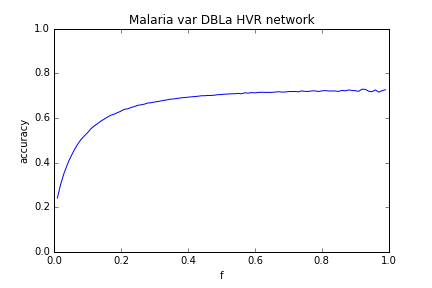
\includegraphics[width=100mm]{images/1a_HVR.png}} \\
	\hline
\end{tabular}
\end{table}
\begin{table}[H]
\centering
\begin{tabular}{|c|c|}
	\hline
	\addheight{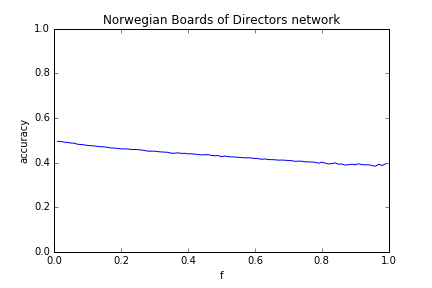
\includegraphics[width=100mm]{images/1a_net1m.png}} \\
	\hline
\end{tabular}
\end{table}

In the Malaria network we can see that as the fraction of observed label increases the accuracy in predicting missing labels increases which implies that there is assortative mixing in the network, because that's when the GbA heuristic works the best. But, still the max accuracy achieved is only about 0.7 which could be attributed to the fact that the node is assigned a label randomly when there is a tie.\\

In the case of Norwegian network, we can see that there is a decrease in the accuracy as the fraction of observed labels increases, which hints us that there isn't much assortative mixing in the network as expected. Which became more conclusive when I visualized the network. The below image is the visualization of the network where the red represents male and blue represents female. We could see that there exists many small individual isolated cliques and can see that females are more central in the network. The number of male-female connections or vice versa is more compared to that of male-male or female-female connections. The above two reasons can be attributed to why the prediction goes wrong when using the GbA heuristic.

\begin{table}[H]
\centering
\begin{tabular}{|c|c|}
	\hline
	\addheight{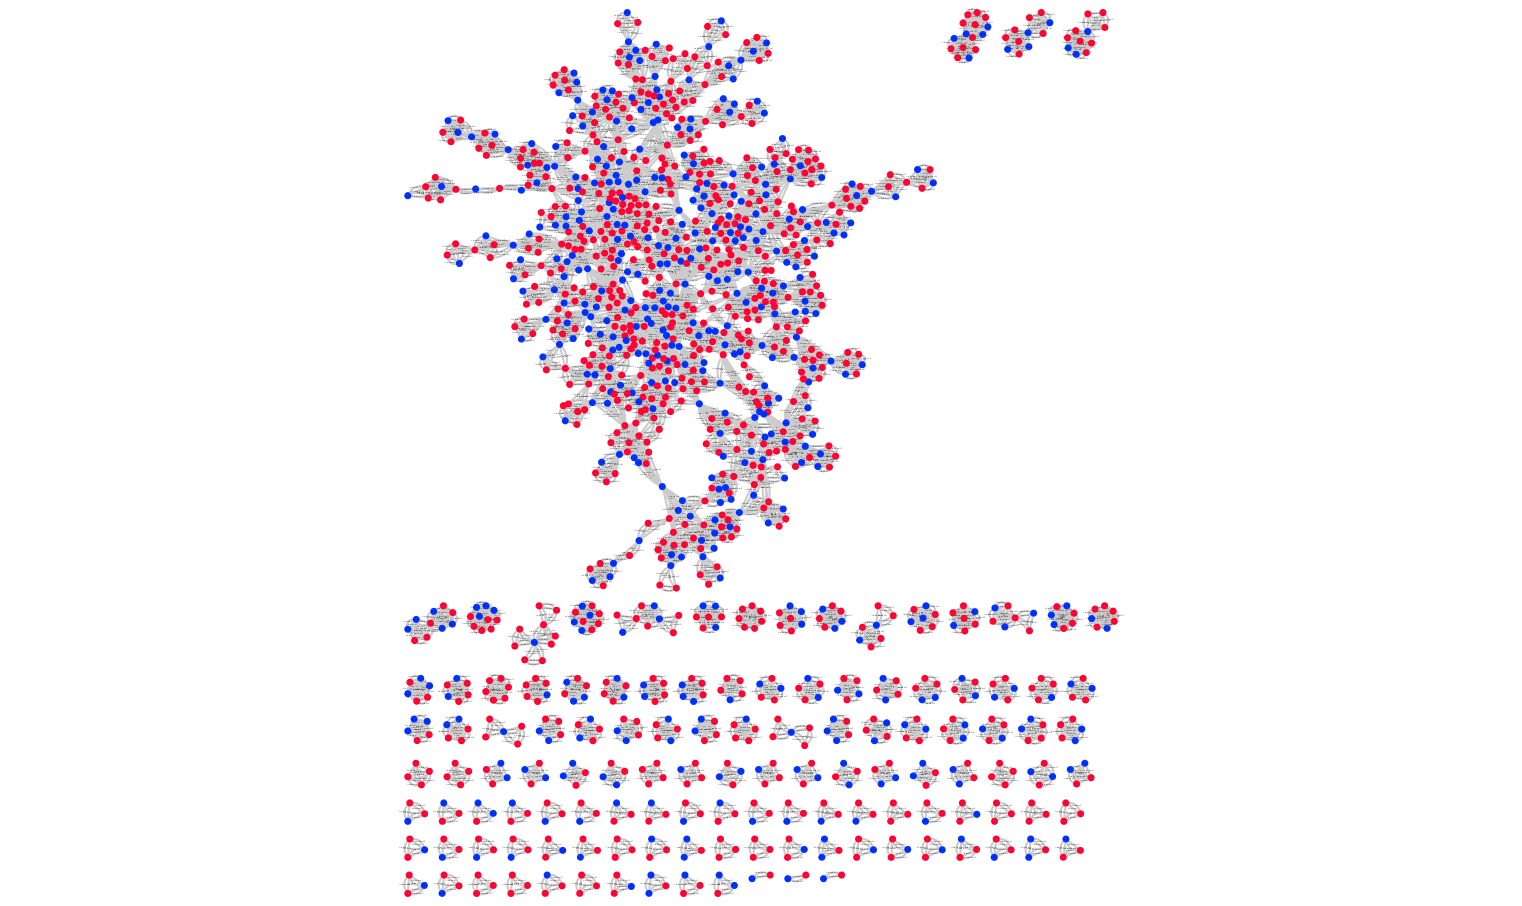
\includegraphics[width=160mm]{images/visual.png}} \\
	\hline
\end{tabular}
\end{table}

\begin{table}[H]
\centering
\begin{tabular}{|c|c|}
	\hline
	\addheight{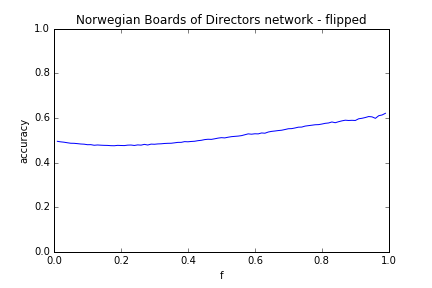
\includegraphics[width=100mm]{images/1a_flip_net1m.png}}\\
	\hline
\end{tabular}
\end{table}

In order to verify the disassortative mixing pattern in the network, I assigned the nodes with missing label a label that is the lowest in the distribution of non-missing labels observed among it's nearest neighbors instead of the mode in the GbA heuristic. The results of it can be seen in the flipped plot above, and we can see that there is an increase in the accuracy as fraction of observed labels increases. 

\newpage
\item
The plots below shows the accuracy defined as AUC of the three heuristics namely degree product, normalized common neighbours, shortest path as a function of the fraction $f \in (0, 1)$ of the edges observed for both the Norwegian Boards of Directors and Malaria var DBLa HVR networks averaged over 100 and 10 iterations for each value of f respectively. We can clearly see that the neighbour and shortest path heuristic perform better than the degree heuristic in predicting the missing edges in both the networks.

\begin{table}[H]
\centering
\begin{tabular}{|c|c|}
	\hline
	\addheight{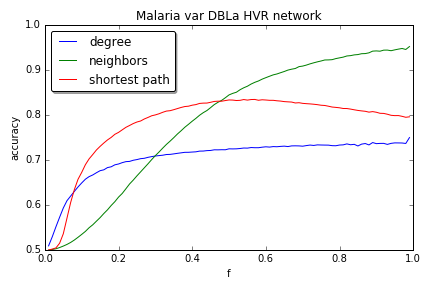
\includegraphics[width=90mm]{images/1b_HVR.png}} \\
	\hline
\end{tabular}
\end{table}
\begin{table}[H]
\centering
\begin{tabular}{|c|c|}
	\hline
	\addheight{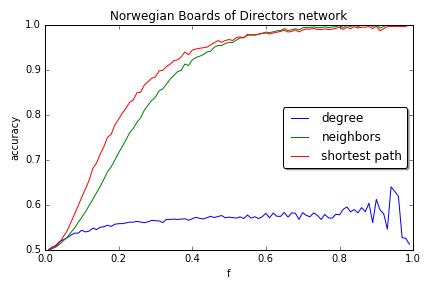
\includegraphics[width=90mm]{images/1b_net1m.png}} \\
	\hline
\end{tabular}
\end{table}

While using the normalized common neighbours heuristic, we can clearly see that the accuracy keeps increasing for both the networks as the fraction of edges considered in the train set increases. This can be attributed to the fact that the malaria network is a single connected component, and the Norwegian network contains many small cliques and a large connected component, so more the number of edges observed more the probability of having common neighbours, and the prediction accuracy increases.\\

While using the shortest path heuristic, we can see that the accuracy increases faster initially and starts stabilizing with further increase in the value of f in the malaria network, whereas the accuracy keeps increasing with the increase in the value of f in the Norwegian network. The behaviour in the Malaria network, can be attributed to the fact that the network is connected, so the accuracy increases rapidly until the emergence of a Giant component in the network and stops increasing after that. But in the case of Norwegian network as it contains many small isolated cliques, so more the number of observed edges better the accuracy in predicting the missing edge.\\

While using the degree product heuristic, we can see that the accuracy increases with the increase in the value of f for both the networks, but the accuracy achieved isn't that great. This heuristic assumes that nodes with higher degree connect with each other. The low accuracy in the Norwegian network is due to the presence of many isolated cliques, as the heuristics assumes that there exists an edge between nodes in different isolated cliques but in reality it doesn't exist. The low accuracy in the Malaria dataset can be attributed to the fact that it becomes difficult to differentiate between the degree product of different pairs after the emergence of giant component.

\end{enumerate}  
\newpage  	
\section*{Problem 2}
The tables below lists the top 10 nodes of the moderately sized Caltech36 and Reed98 networks from the facebook100 network, ordered by their spreading centrality along with their degree.

\begin{table}[H]
\centering
\caption{Caltech36 Network - Transmission Probability 0.023}
\label{Caltech36}
\begin{tabular}{|l|l|l|}
\hline
node\_id & spreading centrality & degree \\
\hline
709      & 269.98               & 248    \\
90       & 256.521              & 203    \\
623      & 255.168              & 160    \\
664      & 255.086              & 184    \\
257      & 253.063              & 172    \\
223      & 252.137              & 194    \\
278      & 251.56               & 171    \\
687      & 251.026              & 160    \\
626      & 246.128              & 156    \\
377		 & 245.254	           & 144    \\
\hline
\end{tabular}
\end{table} 

\begin{table}[H]
\centering
\caption{Reed98 Network - Transmission Probability 0.025}
\label{Reed98}
\begin{tabular}{|l|l|l|}
\hline
node\_id & spreading centrality & degree \\
\hline
679      & 342.011              & 313    \\
873      & 340.101              & 213    \\
889      & 334.342              & 211    \\
646      & 330.438              & 183    \\
147      & 329.819              & 182    \\
328      & 323.153              & 154    \\
562      & 321.744              & 175    \\
230      & 320.066              & 155    \\
293      & 318.884              & 158    \\
236		 & 318.744			   & 154    \\
\hline
\end{tabular}
\end{table} 

From the tables above, we can clearly see that the spreading centrality of a node in a network has a direct dependence on the degree of the node where the epidemic starts. Which implies that, higher the degree of the node which gets infected higher the chances that epidemics spreads and vice versa. It is very much evident in the two networks used, even though the transmission probability is very low for the two networks, still we could see a max of around 40\% of the network being affected when the node that gets infected first is the node with the highest degree.
\newpage
\section*{Code for Problem 1a}
\begin{lstlisting}[language=Python, breaklines=true] 
from __future__ import division
import random
import csv
import networkx as nx
from collections import defaultdict
from collections import Counter

dataPath = "/home/santa/Dropbox/NAM/Problem Set 5/"
files = [("net1m_2011-08-01.txt", "data_people.txt"), ("HVR_5.txt", "metadata_CysPoLV.txt")]
for (filename1, filename2) in files:
    lines = [line.rstrip('\n') for line in open(dataPath+"data/"+filename1)]
    G = nx.Graph()
    for line in lines:
        vertexes = line.split("\t")
        G.add_edge(int(vertexes[0]), int(vertexes[1]))
        G.add_node(int(vertexes[0]))
        G.add_node(int(vertexes[1]))
    
    lines = [line.rstrip('\n') for line in open(dataPath+"data/"+filename2)]
    labels = defaultdict(int)
    
    if filename1.startswith("net1m"):
        for line in lines[1:]:
            node_id = int(line.split(" \"")[0])
            label = int(line.split("\" ")[1])
            if node_id in G.nodes():
                labels[node_id] = label
    else:
        cnt = 1
        for line in lines:
            if cnt in G.nodes():
                labels[cnt] = int(line.strip())
            cnt += 1
    
    labels_set = set(labels.values())
    no_of_iter = 200
    no_of_nodes = G.number_of_nodes()
    fp = open(dataPath+"Code/prob1a_"+filename1.split("_")[0]+".csv", 'a')
    writer = csv.writer(fp)
    writer.writerow(("f", "acc"))
    for f in range(1, 100):
        print f
        f /= 100
        train_size = int(f*no_of_nodes)
        avg_accuracy = 0
        for i in range(no_of_iter):
            train_set = defaultdict(int)
            test_set = defaultdict(int)
    
            while len(train_set) <= train_size:
                key = int(random.choice(labels.keys()))
                train_set[key] = int(labels[key])
    
            for node in G.nodes():
                if not int(node) in train_set:
                    edges = G.edges(node)
                    lst = []
                    for edge in edges:
                        if edge[1] in train_set:
                            lst.append(train_set[edge[1]])
    
                    data = Counter(lst)
                    max_count = 0 if len(data) == 0 else max(data.values())
                    mode = [k for k, v in data.items() if v == max_count]
    
                    if len(mode) == 1:
                        test_set[node] = int(mode[0])
                    else:
                        if len(mode) != 0:
                            test_set[node] = int(random.choice(mode))
                        else:
                            test_set[node] = int(random.sample(labels_set, 1)[0])
    
            cnt = 0
            for key in test_set.keys():
                if test_set[key] == labels[key]:
                    cnt += 1
    
            accuracy = cnt/len(test_set)
            avg_accuracy += accuracy
        writer.writerow((f, (avg_accuracy/no_of_iter)))
    fp.close()

\end{lstlisting}

\begin{lstlisting}[language=Python, breaklines=true]
import matplotlib.pyplot as plt
import pandas as pd

files = ['net1m', 'HVR', 'flip_netm']
title = {}
title['net1m'] = 'Norwegian Boards of Directors network'
title['HVR'] = 'Malaria var DBLa HVR network'
title['flip_net1m'] = 'Norwegian Boards of Directors network - flipped'
for filename in files:
    csv_file = "/home/santa/Dropbox/NAM/Problem Set 5/Code/prob1a_"+filename+".csv"
    df = pd.read_csv(csv_file)
    x = df['f'].tolist()
    y = df['acc'].tolist()
    plt.plot(x, y)
    plt.xlabel('f')
    plt.ylim([0, 1])
    plt.ylabel('accuracy')
    plt.title(title[filename])
    plt.savefig("/home/santa/Dropbox/NAM/Problem Set 5/Latex/images/1a_"+filename+".png")
    plt.clf()
\end{lstlisting}

\section*{Code for Problem 1b}
\begin{lstlisting}[language=Python, breaklines=true]
from __future__ import division
import csv
import random
import networkx as nx
import numpy as np
from sklearn import metrics


def calc_degree_score(graph, u, v, degree_score_set):
    degree = graph.degree(u) * graph.degree(v)
    if degree in degree_score_set:
        degree += random.uniform(0, 1)/no_of_nodes
    return degree


def calc_neighbor_score(graph, u, v, neighbor_score_set):
    i_neighbor = set(graph.neighbors(u))
    j_neighbor = set(graph.neighbors(v))
    union = len(i_neighbor | j_neighbor)
    intersection = len(i_neighbor & j_neighbor)
    neighbor = intersection/union if union != 0 else 0
    if neighbor in neighbor_score_set:
        neighbor += random.uniform(0, 1) / no_of_nodes
    return neighbor


def calc_path_score(graph, u, v, path_score_set):
    try:
        path = 1/nx.shortest_path_length(graph, source=u, target=v)
    except:
        path = 0
    if path in path_score_set:
        path += random.uniform(0, 1) / no_of_nodes
    return path


dataPath = "/home/santa/Dropbox/NAM/Problem Set 5/"
files = [("net1m_2011-08-01.txt", "data_people.txt"), ("HVR_5.txt", "metadata_CysPoLV.txt")]

for (filename1, filename2) in files:
    lines = [line.rstrip('\n') for line in open(dataPath+"data/"+filename2)]
    tot_no_of_nodes = len(lines)
    if filename1.startswith("data"):
        tot_no_of_nodes -= 1
    A_Full = np.zeros(shape=(tot_no_of_nodes, tot_no_of_nodes))
    
    edges = []
    nodes = set()
    lines = [line.rstrip('\n') for line in open(dataPath+"data/"+filename1)]
    for line in lines:
        vertexes = line.split("\t")
        edges.append((int(vertexes[0]), int(vertexes[1])))
        nodes.add(int(vertexes[0]))
        nodes.add(int(vertexes[1]))
        A_Full[int(vertexes[0])-1][int(vertexes[1])-1] = 1
        A_Full[int(vertexes[1])-1][int(vertexes[0])-1] = 1
    no_of_edges = len(edges)
    node_list = list(nodes)
    no_of_nodes = len(node_list)
    
    fp = open(dataPath+"Code/prob1b_"+filename1.split("_")[0]+".csv", "wt")
    writer = csv.writer(fp)
    writer.writerow(("f", "d", "n", "p"))
    fp.close()
    
    no_of_iter = 10
    for f in range(1, 100):
        print f
        f /= 100
        train_size = int(f*no_of_edges)
        degree_accuracy = 0
        neighbor_accuracy = 0
        path_accuracy = 0
    
        for itr in range(no_of_iter):
            train_set = random.sample(edges, train_size)
            G = nx.Graph()
            G.add_edges_from(train_set)
            G.add_nodes_from(node_list)
            A = np.zeros(shape=(tot_no_of_nodes, tot_no_of_nodes))
            for (x, y) in train_set:
                A[x-1][y-1] = 1
                A[y-1][x-1] = 1
            
            y_true = []
            y_degree_score = []
            y_degree_score_set = set()
            y_neighbor_score = []
            y_neighbor_score_set = set()
            y_path_score = []
            y_path_score_set = set()
    
            for x in range(0, no_of_nodes):
                i = node_list[x]
                for y in range(x+1, no_of_nodes):
                    j = node_list[y]
                    if A[i-1][j-1] == 0:
                        if A_Full[i-1][j-1] == 1:
                            y_true.append(1)
                        else:
                            y_true.append(0)
    
                        degree_score = calc_degree_score(G, i, j, y_degree_score_set)
                        y_degree_score.append(degree_score)
                        y_degree_score_set.add(degree_score)
    
                        neighbor_score = calc_neighbor_score(G, i, j, y_neighbor_score_set)
                        y_neighbor_score.append(neighbor_score)
                        y_neighbor_score_set.add(neighbor_score)
    
                        path_score = calc_path_score(G, i, j, y_path_score_set)
                        y_path_score.append(path_score)
                        y_path_score_set.add(path_score)
    
            y_degree_score = np.asarray(y_degree_score)
            y_degree_score /= sum(y_degree_score)
            y_neighbor_score = np.asarray(y_neighbor_score)
            y_neighbor_score /= sum(y_neighbor_score)
            y_path_score = np.asarray(y_path_score)
            y_path_score /= sum(y_path_score)
    
            degree_accuracy += metrics.roc_auc_score(y_true, y_degree_score)
            neighbor_accuracy += metrics.roc_auc_score(y_true, y_neighbor_score)
            path_accuracy += metrics.roc_auc_score(y_true, y_path_score)
    
        fp = open(dataPath+"Code/prob1b_"+filename1.split("_")[0]+".csv", "a")
        writer = csv.writer(fp)
        writer.writerow((f, (degree_accuracy/no_of_iter), (neighbor_accuracy/no_of_iter), (path_accuracy/no_of_iter)))
        fp.close()

\end{lstlisting}

\begin{lstlisting}[language=Python, breaklines=true] 
import matplotlib.pyplot as plt
import pandas as pd

files = ['net1m', 'HVR']
title = {}
title['net1m'] = 'Norwegian Boards of Directors network'
title['HVR'] = 'Malaria var DBLa HVR network'
for filename in files:
    csv_file = "/home/santa/Dropbox/NAM/Problem Set 5/Code/prob1b_"+filename+".csv"
    df = pd.read_csv(csv_file)
    x = df['f'].tolist()
    plt.plot(x, df['d'].tolist(), label='degree')
    plt.plot(x, df['n'].tolist(), label='neighbors')
    plt.plot(x, df['p'].tolist(), label='shortest path')
    plt.xlabel('f')
    plt.ylim([0.5,1])
    plt.ylabel('accuracy')
    plt.title(title[filename])
    plt.legend(loc='upper left', fancybox=True, shadow=True)
    plt.tight_layout()
    plt.savefig("/home/santa/Dropbox/NAM/Problem Set 5/Latex/images/1b_"+filename+".png")
    plt.clf()
\end{lstlisting}

\section*{Code for Problem 2 - EC}
\begin{lstlisting}[language=Python, breaklines=true] 
from __future__ import division
import random
import networkx as nx
import csv
from collections import defaultdict

dataPath = "/home/santa/Dropbox/NAM/Problem Set 5/"
files = ["Caltech36", "Reed98"]
for filename in files:
    lines = [line.rstrip('\n') for line in open(dataPath+"data/"+filename+".txt")]
    G = nx.Graph()
    for line in lines:
        vertexes = line.split("\t")
        G.add_edge(vertexes[0], vertexes[1])
    avg_deg = sum(list(G.degree(G.nodes()).values()))/G.number_of_nodes()
    p = 1/avg_deg
    no_of_iter = 1000
    
    f = open(dataPath+"Code/"+filename+".csv", 'a')
    writer = csv.writer(f)
    writer.writerow(("node_id", "spreading centrality", "degree"))
    for i in G.nodes():
        print i
        epidemic_size = 0
        for j in range(no_of_iter):
            infected_list = defaultdict(int)
            infected_list[i] = 1
            lst = [i]
            while len(lst):
                newList = []
                for infected_node in lst:
                    edges = G.edges(infected_node)
                    for edge in edges:
                        if random.uniform(0, 1) <= p:
                            if infected_list[edge[1]] != 1:
                                newList.append(edge[1])
                                infected_list[edge[1]] = 1
                lst = newList
            epidemic_size += len(infected_list)
        writer.writerow((i, (epidemic_size/no_of_iter), G.degree(i)))
    f.close()
\end{lstlisting}
\end{document}
